% -*- TeX-master: "paper.tex"; TeX-PDF-mode: t; ispell-local-pdict: "words" -*-

% drm119 and drm120
% * HP ProLiant DL580 G5
% * EMC CLARiiON CX3-40

% 400G LUN
% * 5-disk RAID-5 (64K stripe)

\long\def\ignore#1{}

\section{Evaluation}
\label{sec:evaluation}

In this section, we present results from the evaluation of our
deduplication techniques using various microbenchmarks and realistic
workloads.  We begin in Section~\ref{sec:vmware-vdi-analysis} with
experiments and analysis that shows the space savings achievable with
deduplication as well as the space overheads introduced by it, using
data from a real corporate VDI deployment. We also draw a comparison
against linked clones, an alternative way of achieving space savings.

We have implemented a functional prototype of \DeDe atop VMware
VMFS. Although we haven't spent any significant time optimizing it, it
is worthwhile examining its basic performance characteristics. In
Section~\ref{sec:run-time-overheads}, we present the run-time
performance impact of write monitoring and other changes to the file
system introduced by deduplication, as well as the run-time
performance gained from improved cache locality.  Finally,
we look at the performance of the deduplication process itself in
Section~\ref{sec:dedup-rate}.


\subsection{Analysis of Virtual Disks in the Wild}
\label{sec:vmware-vdi-analysis}

To evaluate the usefulness of deduplication in our target workload
segment of VDI, we analyzed the virtual disks from a production
corporate VDI cluster serving desktop VMs for approximately 400 users
on top of a farm of 32 VMware ESX hosts.  Out of these, we selected
113 VMs at random to analyze for duplicate blocks, totaling 1.3~TB of
data (excluding blocks consisting entirely of NULL bytes).  Each user
VM belonged exclusively to a single corporate user from a
non-technical department like marketing or accounting.  The VMs
have been in use for six to twelve months and all
originated from a small set of standardized Windows~XP images.  From
our experience, this is typical for most enterprise IT organizations,
which limit the variation of operating systems to control management
and support costs.
%
%% To avoid interruption of service, our tool took a live snapshot of the
%% users' virtual machines but otherwise avoided shutting down these
%% VMs. A snapshot operation results in the base virtual disk becoming
%% read-only so that we had a stable file to read from. Our tool computed
%% and saved away \shaone hashes of the virtual disk data at the
%% granularity of 512-bytes. We then put these together to form
%% signatures at various block granularities.
%

Figure~\ref{fig:vmware-it-vdi-bar} shows the reduction in storage
space for this VDI farm using deduplication block sizes between 4~KB
and 1~MB. As expected, VDI VMs have a high degree of similarity,
resulting in an $\sim$80\% reduction in storage footprint for the 4~KB
block size, which falls off logarithmically to $\sim$35\% for 1~MB
blocks.  Deduplication at the 4~KB block size reduces the
original 1.3~TB of data to 235~GB.  Given the significant advantage of
small block sizes, we chose to use a default 4~KB block size
for \DeDe.  However, a reasonable argument can be made for the smaller
metadata storage and caching overhead afforded by an 8~KB block size.
We are exploring this as well as dynamic block size selection as
future work.

% This data set exhibits a high degree of duplication because the VMs
% all originated from a small set of standardized Windows~XP images.
% From our experience, this is typical for most enterprise IT
% organizations, which limit the variation of operating systems to control
% management and support costs.  For privacy reasons, we were
% not permitted to inspect the VM file systems more
% closely to determine the most common causes of duplication.

Figure~\ref{fig:vmware-it-vdi-cdf} shows a CDF of the same data,
detailing the duplication counts of individual blocks in terms of
the number of references to each block in the file
system \emph{after} deduplication.  For example, at the 4~KB block
size, 94\% of deduplicated blocks are referenced 10 or fewer times by
the file system (equivalently, 6\% of deduplicated blocks are
referenced more than 10 times).  Thus, in the original data, most
blocks were duplicated a small number of times, but there was a very
long tail where some blocks were duplicated many times.  At the very
peak of the 4~KB distribution, some blocks were duplicated over
100,000 times.  Each of these blocks individually represented over
400~MB of space wasted storing duplicate data. Overall, this data
serves to show the potential for space savings from deduplication in
VDI environments.

%%%%%%%%%%%%%%%%%%%%%%%
%%%% Figure %%%%%%%%%%%
%%%%%%%%%%%%%%%%%%%%%%%

\begin{figure}[t]
\centering
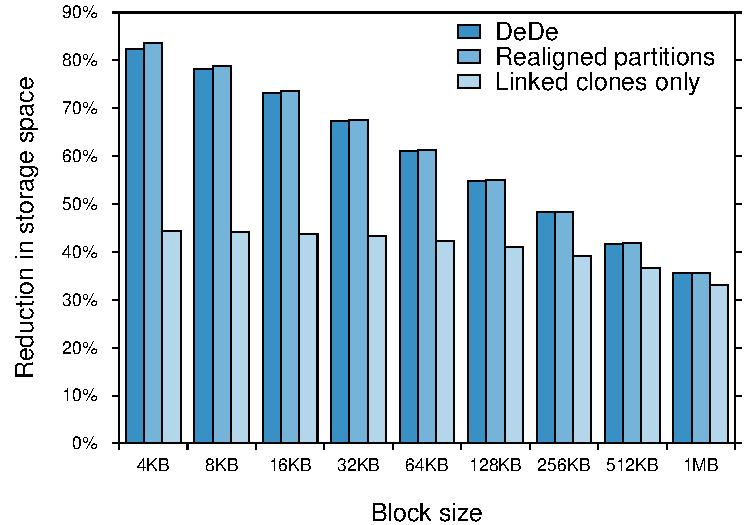
\includegraphics[scale=0.6]{figures/vmware-it-vdi-bar2.pdf}
%\vspace{-0.2in}
\caption{Duplication available at various block sizes and for
  different variations on the approach. Data is from a
  production VDI deployment of 113 Windows XP VMs.}
%\vspace{-0.1in}
\label{fig:vmware-it-vdi-bar}
\end{figure}

%%%%%%%%%%%%%%%%%%%%%%%
%%%% /Figure %%%%%%%%%%
%%%%%%%%%%%%%%%%%%%%%%%

%%%%%%%%%%%%%%%%%%%%%%%
%%%% Figure %%%%%%%%%%%
%%%%%%%%%%%%%%%%%%%%%%%

\begin{figure}[t]
\centering
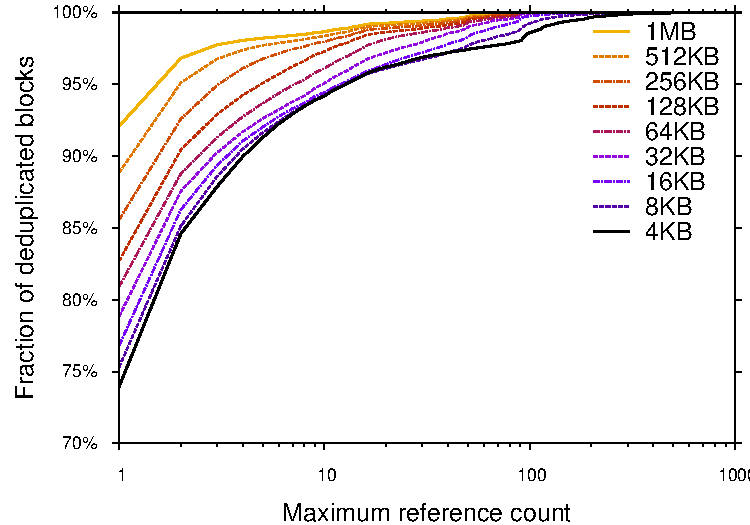
\includegraphics[scale=0.6]{figures/vmware-it-vdi-cdf.pdf}
%\vspace{-0.2in}
\caption{CDF of block duplication counts.  A few blocks occur over
  100,000 times. Data is from the same deployment as shown in
  Figure~\ref{fig:vmware-it-vdi-bar}.}
\vspace{-0.1in}
\label{fig:vmware-it-vdi-cdf}
\end{figure}

%%%%%%%%%%%%%%%%%%%%%%%
%%%% /Figure %%%%%%%%%%
%%%%%%%%%%%%%%%%%%%%%%%

\subsubsection{Space Overheads}

While \DeDe reduces the amount of space required by file data, it
requires additional space for both the index and the additional
metadata introduced by mixed block sizes.  For our VDI data set, at a
4~KB block size, this additional data totaled 2.7~GB, a mere $1.1\%$
overhead beyond the deduplicated file data.

\ignore{
  ;; Evaluate this after the other two
  (let* ((total-gb (+ total-index-gb total-metadata-gb))
         (overhead (/ total-gb 235)))
    (list total-gb (* 100 overhead)))
}

The index represented 1.5~GB of this overhead, 194~MB of which was
file system metadata (pointer blocks) for the virtual arena.
The size of the index scales linearly with the size of
the deduplicated data because each deduplicated block has one index
entry.  However, its relative overhead does vary with the ratio of
unique to shared
blocks, because shared blocks require 4 bytes to locate plus virtual
arena metadata, while unique blocks require 12 bytes beyond the
18~bytes required on average for each entry's header and hash.
However, even in the worst case, the index represents only $0.73\%$ 
overhead.

\XXX[The expected size of each index entry, given $n$ total entries
and a fraction $s$ of shared entries is \[1 + \lceil20 -
\nicefrac{1}{8}\log_2(n)\rceil + 4s + 12(1-s)\]]

\ignore{
(let* ((data-gb 235)                    ; GB of data *post* dedup
       (pct-shared 0.824)               ; % shared entries
;;       (pct-shared 0.0)                 ; Worse case

       (entries (* data-gb 1024 256))   ; # of index entries
       (header 1)                       ; Header bytes per entry
       (hash                            ; Hash bytes per entry
        (fceiling (- 20 (/ (log entries 2) 8))))
       (payload                         ; Payload bytes per entry
        (+ (* pct-shared 4) (* (- 1 pct-shared) 12)))
       (entry-bytes (+ header hash payload))
       (index-bytes                     ; Index size (bytes)
        (* entries entry-bytes))
       (index-gb (/ index-bytes 1024 1024 1024)) ; Index size (GB)
       (ratio (/ index-gb data-gb))              ; Ratio index to data

       (arena-entries (* entries pct-shared))
       (arena-fpbs (/ arena-entries 256))
       (arena-pbs (/ arena-fpbs 1024))
       (arena-kb (+ 4 (* arena-pbs 4) (* arena-fpbs 1)))
       (arena-mb (/ arena-kb 1024))
       (arena-gb (/ arena-mb 1024))

       (index+arena-gb (+ index-gb arena-gb))
       (index+arena/deduped-data (/ index+arena-gb data-gb)))
  (defvar total-index-gb index+arena-gb)
  (defvar avg-bytes/entry entry-bytes)
  `(index+arena-gb ,index+arena-gb
    index+arena/deduped-data ,index+arena/deduped-data
    ,(+ header hash) ,arena-mb))
}

\XXX[The percentage of index size relative to the total data size
remains essentially constant with $n$.  Varying $s$ between $0$ and
$1$ varies the percentage between $0.73\%$ and $0.54\%$, respectively.]

% entries(dgb)=dgb*1024*256
% esize(n,s)=1+ceil(20-(log(n)/log(2))/8)+4*s+12*(1-s)
% ratio(dgb,s)=entries(dgb)*esize(entries(dgb),s)/1024/1024/1024/dgb

Prior to deduplication, file metadata (inodes and pointer blocks)
represented a mere $0.0004\%$ overhead, owing to the efficiency of
tracking VMFS's 1~MB file blocks.  After deduplication, each 1~MB
block that was divided into sub-blocks requires a new pointer block at
1~KB apiece.  As a result, metadata overhead increased to $0.49\%$
after deduplication, or
1.1~GB of data in total.  While this is a dramatic increase, metadata
is still a very small fraction of the overall space.

\ignore{
(let* ((data-gb 1346.334)               ; *Pre* dedup data size
       (pct-fragged 0.8697)
       (dedup-gb 234.59)                ; *Post* dedup total

       (pbs (+ 1 data-gb))
       (fpbs (* data-gb 1024))
       (md-regular (* 4096 pbs))
       (md-fragged (+ md-regular (* 1024 fpbs pct-fragged)))
       (data-bytes (* data-gb 1024 1024 1024))
       (dedup-bytes (* dedup-gb 1024 1024 1024))
       (md/total-regular (/ md-regular (+ md-regular data-bytes)))
       (md/total-fragged (/ md-fragged (+ md-fragged data-bytes)))
       (md/dedup-fragged (/ md-fragged (+ md-fragged dedup-bytes)))
       (pre-overhead (/ md-regular data-bytes))
       (post-overhead (/ md-fragged dedup-bytes))
       (new-gb (/ (- md-fragged md-regular) 1024 1024 1024)))
  (defvar total-metadata-gb new-gb)
  (list md-regular md-fragged new-gb
        (* 100 md/total-regular)
        (* 100 md/total-fragged)
        (* 100 md/dedup-fragged)
        (* 100 pre-overhead)
        (* 100 post-overhead)))
}

\subsubsection{Partition Alignment Issues}

Our approach of dividing disks into fixed size blocks is sensitive to
the alignment of data on those disks.  Unfortunately, for historical
reasons, the first partition of partition tables created by utilities
like {{\tt \small fdisk}} on commodity PC systems has a start address
512~bytes short of a 4~KB boundary, which can in turn cause all
logical file system blocks to straddle 4~KB disk block boundaries.
This has well-known negative performance effects~\cite{vmware-align},
particularly for storage array caches, which are forced to fetch two
blocks for each requested file system block.  We were initially
concerned that this partition misalignment could negatively impact
deduplication opportunities, so we ``fixed'' the alignment of our VDI
data by shifting all of the virtual disks by 512~bytes.
Figure~\ref{fig:vmware-it-vdi-bar} compares the results of
deduplication with and without this realignment and shows that, in
practice, partition alignment actually had very \emph{little} impact
on achieved deduplication. \XXX[Austin][... , a result observed in
previous work as well~\cite{rhea-foundation}.  It's unclear they're
actually referring to this problem or concluding that it's not a
problem in practice.]  While this may still prove to be a problem for
well-aged guest file systems, if necessary, it can be solved in a
virtualized environment by padding the virtual disk image file to
realign the guest file system blocks with the host file system blocks.

% The descriptor format for VMware's virtual disk images supports
% multiple extents. Our technique is to shift the virtual disk logical
% block address range down 4~KB~--~512~bytes and put those 3584~bytes
% in another small extent. For existing VMs, this can be done online
% by performing a transparent data migration whereas new VMs would
% benefit from this from the start. We would like to avoid making
% assumptions about guest block size so would actually shift
% 1~MB--~512~bytes to avoid block size cadence mismatch problems.

\subsubsection{Deduplication Versus Linked Clones}
\label{sec:vmware-vdi-linked-clones}

\emph{Linked clones} are a simpler space saving alternative to
deduplication where individual user VMs are initially constructed as
block-level COW snapshots of a golden master VM.  This uses the same COW
mechanism as \DeDe, but all sharing happens during VM creation and the
user VM images strictly diverge from the base disk and from each other
over time.

% a structured, a priori form the deduplication

In order to compare the efficacy of linked clones versus full
deduplication, we simulated the structured sharing of linked clones on
our VDI data set.  This comparison was necessarily imperfect because
we had access to neither the base disks nor ancestry information for
the VDI VMs, but it did yield a \emph{lower bound} on the total space
required by linked clones.  The analysis used our regular
deduplication algorithm but restricted it to deduplicating blocks only
when they were at the same offset in two files, a reasonable
approximation to user disks that are a minimal delta from the
base disk (\eg, no security patches or software updates have been
installed in the user disks).

Figure~\ref{fig:vmware-it-vdi-bar} compares the savings achieved by
linked clones against those achieved by \DeDe, again at various COW
block sizes.  Linked clones max out at a $44\%$ reduction in space,
reducing the 1.3~TB of original data to 740~GB, a storage requirement
over three times larger than full deduplication achieved.
% (/ 194070820 61497555.0)

% An alternate way of achieving storage space reduction is to design it
% into the virtual disk file usage pattern. Linked clones are one such
% scheme where a single base disk is used for all VMs in the
% setup. Writes are handled by COWing data blocks to new locations. The
% specialized blocks can be stored in separate files or the file system
% can be designed to internally and transparetly support this
% functionality (\eg, NetApp's WAFL or block-level COW in VMFS). The
% block size granularity at which this functionality is implemented has
% performance implications both for the COW operation as well as for the
% level of achieved storage efficiency. Let's take the example of
% block-level COW support in VMFS which typically has a 1~MB block size:
% a single sector write to a block would result in reading in the entire
% 1~MB, modifying it in memory and rewriting it to a new
% location.\XXX[Irfan][R-M-W was used here: I think that term is
% confusing in this context, see wikipedia]. In other words, the
% specialization operation is granular only down the file system block
% size. With large block sizes, for any arbitrarily chosen block, the
% probability is higher that the guest file system may write to some
% portion of it. This in turn implies a higher storage footprint over
% time.

% To test this, we decided to use our existing data from the previous
% section.  We compute deduplication statistics assuming blocks can only
% be deduplicated if they are at the same offset in two files--they key
% difference between \DeDe and linked clones.  This is a way of upper
% bounding the savings that linked clones could yield for the files.
% This bound is loosened by two things: (1) If a block was {\it ever}
% written to, it would not be shared by linked clones, even if, say, it
% was written to a second time to change it back, or some other VM wrote
% the same thing to the equivalent block in that VM.  Since we have no
% idea which blocks have or have not been modified from the base image,
% we have to give linked clones the benefit of the doubt in this case.
% (2) One VM can only inherit from one base disk, but computing the
% optimal set of base disks is infeasible.  For example, consider four
% VMs $A-D$, each containing two blocks 1 and 2.  If $A_1=B_1$ and
% $C_1=D_1$, then for block 1, we consider $A$ and $B$ as sharing a base
% disk and $C$ and $D$ as sharing a base disk.  However, suppose that
% for block 2, $A_2=C_2$ and $B_2=D_2$.  For this block, we consider $A$
% and $C$ as sharing a base disk and $B$ and $D$ as sharing a base disk.
% Linked clones cannot satisfy both cases at once, but it is
% computationally infeasible for us to compute what the best set of base
% disks should have been so we give linked clones the benefit of doubt.

\subsection{Run-time Effects of Deduplication}
\label{sec:run-time-overheads}

\DeDe operates primarily out of band and engenders no slowdowns for
accessing blocks that haven't benefited from deduplication. It can
also improve file system performance in certain workloads by reducing
the working set size of the storage array cache. For access to
deduplicated blocks, however, in-band write monitoring and the effects
of COW blocks and mixed block sizes can impact the regular performance
of the file system.  Unless otherwise noted, all of our measurements
of the run-time effects of deduplication
were performed using Iometer~\cite{iometer} in a virtual machine
stored on a 400~GB 5-disk RAID-5 volume of an EMC CLARiiON CX3-40
storage array.

\subsubsection{Overhead of In-Band Write Monitoring}
\label{sec:eval-sha-1}

Since \DeDe's design is resilient to dropped write log entries, if the
system becomes overloaded, we can shed or defer the work of in-band
hash computation based on user-specified policy. Still, if write
monitoring is enabled, the hash computation performed by \DeDe on
every write IO can represent a non-trivial overhead.

% We measured the cost of the \shaone computation of a 64~KB write block
% to be $\sim$470~microseconds on an Intel Xeon CPU 5160 running @
% 3.00GHz.
To understand the worst-case effect of this, we ran a write-intensive
workload with minimal computation on a 5~GB virtual disk.
Table~\ref{table:sha1} shows that these worst case effects can be
significant. For example, for a 100\%
sequential, 100\% write workload, the CPU overhead was 6.6$\times$
that of normal at the same throughput level. However, because VMware ESX
Server offloads the execution of the IO issuing path code, including
the hash computation, onto idle processor cores, the actual IO
throughput of this workload was unaffected.

\begin{table}
\footnotesize
%\small
%HEVEA \small
% XXX The text *should* have been small in LaTeX
\centering
\addtolength{\tabcolsep}{-2.2pt}
\begin{tabular}{|p{1.2cm}||c|c|c||c|c|c|}
\hline
 \%- & \multicolumn{3}{c||}{Baseline} &\multicolumn{3}{c|}{\DeDe}\\
 Sequential & {\it T} (MB/s) &  {\it L} (ms) & CPU & {\it T} (MB/s) & {\it L} (ms) & CPU\\
\hline \hline
  100\%    & 233 & 8.6 & 33\% & 233  & 8.6 & 220\% \\
    0\%    & 84  & 24  & 16\% & 84   & 24  & 92\%  \\
\hline
\end{tabular}
\caption{Overhead of in-band write monitoring on a pure IO
  workload. Results are in
  terms of throughput ({\it T}) and latency ({\it L}) for Iometer
  issuing 32 outstanding 64~KB IOs to a 5~GB virtual disk.
  The CPU column denotes the utilized processor time relative to a
  single core.}
\label{table:sha1}
\end{table}

\begin{table}
%\footnotesize
\small
\centering
\addtolength{\tabcolsep}{-2pt}
\begin{tabular}{|c|c|c|c|c|}
\hline
  & Baseline & \scriptsize{Error} & \shaone & \scriptsize{Error} \\
\hline \hline
Operations/Min     & 29989  & 1.4\% & 29719 & 0.8\%   \\
Response Time (ms) & 60 ms  & 0.8\% & 61ms  & 1.4\%     \\
\hline
\end{tabular}
\caption{Overhead of in-band write monitoring on a SQL Server
  database VM running an online e-commerce application. The mean
  transaction rate (operations/min) and response times for 10 runs are
  within noise for this workload. The reported ``error'' is standard
  deviation as a percentage of mean.}
\label{table:sha1-dvdstore}
\end{table}

We don't expect the effect of the additional computation to be a
severe limitation in realistic workloads, which, unlike our
microbenchmark, perform computation in addition to IO.  To illustrate
this, we ran
the in-band \shaone computation on a realistic enterprise workload. We
experimented with a Windows Server 2003 VM running a Microsoft SQL
Server 2005 Enterprise Edition database configured with 4 virtual
CPUs, 6.4~GB of RAM, a 10~GB system disk, a 250~GB database disk, and
a 50~GB log disk.  The database virtual disks were hosted on an 800~GB
RAID-0 volume with 6 disks; log virtual disks were placed on a 100~GB
RAID-0 volume with 10 disks.  We used the Dell DVD store (DS2)
database test suite~\cite{dvdstore}, which implements a complete
online e-commerce application, to stress the SQL database and measure
its transactional throughput and latency.  The DVD
Store workload issues random 8~KB IOs with a write/read ratio of 0.25,
and a highly variable number of outstanding write IOs peaking around
28~\cite{srs-vpact09}.  Table~\ref{table:sha1-dvdstore} reports a
summary of overall application performance with and without the
in-band \shaone computation for writes. For this workload, we
observed no application-visible performance loss, though extra CPU
cycles on other processor cores were being used for the hash
computations.

\subsubsection{Overhead of COW Specialization}

Writing to a COW block in VMFS is an expensive operation, though the
current implementation is not well optimized for the COW sub-blocks
used extensively by \DeDe.  In our prototype, it takes $\sim$10~ms to
specialize a COW block, as this requires copying its content into a
newly allocated
block in order to update it.  As such, any workload phase shift where a
large set of previously deduplicated data is being specialized will
result in significant performance loss.  However, in general, we
expect blocks that are identical between VMs are also less likely to
be written to and, unlike most approaches to deduplication, we do not
suffer this penalty for writes to unique blocks.  Optimizations to
delay sharing until candidate blocks have been ``stable'' for some
length of time may help further mitigate this overhead, as suggested
in~\cite{hong04sandedup}.

% Based on the assumption that blocks that have not been written to for
% a long time are less likely to be written to in the near future, it
% may be possible to further mitigate the overhead of COW specialization
% by postponing block sharing until both candidates have been ``stable''
% for some length of time, as suggested in~\cite{hong04sandedup}.

\subsubsection{Overhead of Mixed Block Sizes}
\label{sec:eval-mixed}

VMFS's 1~MB file blocks permit very low overhead translation from
virtual disk IO to operations on the physical disk.  While the mixed
block size support we added to VMFS is designed to
retain this efficiency whenever 1~MB blocks can be used, it
unavoidably introduces overhead for 4~KB blocks from traversing the
additional pointer block level and increased external
fragmentation.

To measure the effects of this, we compared IO to two 5~GB virtual
disks, one backed entirely by 1~MB blocks and one backed entirely by
4~KB blocks.  These configurations represent the two extremes of
deduplication: all unique blocks and all shared blocks, respectively.
The first disk required one pointer block level and was broken into 3
separate extents on the physical disk, while the second disk required
two pointer block levels and spanned 163 separate extents.

\iffalse
% This table was with start of VMFS partition unaligned.
\begin{table}
  \small
  \centering
  \begin{tabular}{|c|c|c|c|}
    \hline
    Workload & \multicolumn{2}{|c|}{Peak throughput (MB/s)} & Overhead \\
    & \parbox[t]{1.3cm}{\centering 1~MB} & \parbox[t]{1.3cm}{\centering 4~KB} & \\
    \hline\hline
    % 8 OIOs
    % (- 1 (/ 149.0 241))
    % Latency 1MB 2.1  4K 3.3
%   100\% & Writes & 241 & 149  & 38\% \\

    % 48 OIOs
    % (- 1 (/ 148.0 246))
    % Latency 1MB   4K 20.3
    Sequential write & 246 & 148  & 40\% \\

    % 48 OIOs
    % (- 1 (/ 60.0 69))
    % Latency 1BM 43 4K 49
    Random write & 69 &  60 & 13\% \\

    % 48 OIOs
    % (- 1 (/ 32.0 52))
    % Latency 1MB 58.1, 4K 92
    Sequential read & 52 & 32 & 38\% \\

    % 48 OIOs
    % (- 1 (/ 39.0 44))
    % Latency 1MB 67.9, 4K 44.1
    Random read & 44 & 39 & 11\% \\
    \hline
  \end{tabular}
  \caption{Overhead of Mixed Block
    Fragmentation. Peak throughput achieved for 64~KB sequential and
    random workloads compared between two virtual disks, one backed by
    1~MB blocks and another by 4~KB blocks. In the 4~KB case, number of
    disjoint fragments of the virtual disk file is 163 which implies
    an average sequential run of 31~MB on
    average.}
  \label{table:mixed-block-overhead}
\end{table}
\fi

\iftrue
% This table was with start of VMFS partition aligned to 128 sectors or 64KB.
\begin{table}
  \small
  \addtolength{\tabcolsep}{-2pt}
  \centering
  \begin{tabular}{|c|c|c|c|c|}
    \hline
    \% Sequential & IO Type & \multicolumn{2}{|c|}{Throughput (MB/s)} & Overhead \\
    & & \parbox[t]{1.15cm}{\centering BS=1~MB} & \parbox[t]{1.15cm}{\centering BS=4~KB} & \\
    \hline\hline
    % 16 OIOs
    % Latency 1MB 4.2  4K 6.7
    100\% & Writes & 238 & 150  & 37\% \\

    % 16 OIOs
    % Latency 1MB 15 4K 16.6
    0\% & Writes & 66 &  60 & 9\% \\

    % 16 OIOs
    % Latency 1MB 4.1  4K 7.4
    100\% & Reads & 245 & 135 & 45\% \\

    % 16 OIOs
    % Latency 1MB 27 4K 31
    0\% & Reads & 37  & 32 & 14\% \\
 \hline
\end{tabular}
\caption{Overhead of mixed block
    fragmentation. Throughput achieved for 64~KB sequential and random
    workloads with 16 outstanding IOs. The comparison is between two
    virtual disks backed by block sizes (BS) of 1~MB and 4~KB,
    respectively. In the 4~KB case, the virtual disk file consists of
    163 disjoint fragments, which implies a sequential run of
    31~MB on average.}
\label{table:mixed-block-overhead}
\end{table}

\else

\begin{table}
  \small
  \addtolength{\tabcolsep}{-2pt}
  \centering
  \begin{tabular}{|c|c|c|c|}
    \hline
    \% Sequential & \multicolumn{2}{|c|}{Peak throughput (MB/s)} & Overhead \\
    & \parbox[t]{1.3cm}{\centering 1~MB} & \parbox[t]{1.3cm}{\centering 4~KB} & \\
    \hline\hline
    % 8 OIO's is peak for sequential
    % (- 1 (/ 36.0 52))
    100\% & 52 & 36 & 31\% \\
    % 48 OIO's is peak for random
    % (- 1 (/ 29.0 37))
    50\% & 37 & 29 & 22\% \\
    \hline
  \end{tabular}
    \caption{Peak throughput achieved for sequential and random
    workloads compared between two virtual disks, one backed by 1~MB
    blocks and another by 4~KB blocks.}
  \label{table:mixed-block-overhead}
\end{table}

\fi

The results of reading from these virtual disks are summarized in
Table~\ref{table:mixed-block-overhead}.  Unfortunately, sub-blocks
introduced a non-trivial overhead for sequential IO.  This is partly
because VMFS's sub-block placement and IO handling is not yet
well-optimized since sub-blocks have not previously been used in the
VM IO critical path, whereas VMFS's file block IO has been heavily
optimized.  One possible way to mitigate this overhead is by
preventing the deduplication process from subdividing file blocks
unless they contain some minimum number of 4~KB candidates for
sharing.  This would impact the space savings of deduplication, but
would prevent \DeDe from subdividing entire file blocks for the sake
of just one or two sharable blocks.  Improvements in sub-block IO
performance and block subdivision are considered future work.

% Table~\ref{table:fragment} shows data for read and write IOs with
% various other workload parameters. We can see that in each case,
% fragmentation has a large negative effect in throughput for these
% workloads\XXX[Irfan][Revisit after rerunning this experiment with
% Murali's new changeset]. The typical
% %VDI 
% workloads that \DeDe targets don't experience a lot of sequential IO
% so in practice with real applications, we expect this effect to be
% minimal. Indeed for already random workloads, an increase in
% fragmentation is not expected to give worse performance. Furthermore,
% by removing duplicated entries, the disk array cache footprint is
% reduced which may help mitigate the negative performace effects of
% reduced spatial locality.  It is important to note that throughput
% won't be affected for workloads that are not
% deduplicated.  \XXX[Irfan][Explain whether the level of fragmentation
% in our experiment is typical or not.]

\XXX[
\begin{notes}
  \begin{itemize}
     \item Microbenchmark to exercise the overhead of extra metadata traversal
     \item Random data as fast as possible?
  \end{itemize}
\end{notes}
]

\iffalse
\begin{table*}
\small
\centering
%\addtolength{\tabcolsep}{-2pt}
\begin{tabular}{|p{1.7cm}|c|p{1.2cm}|p{1.5cm}|p{1.5cm}|p{1.5cm}||p{1.5cm}|p{1.5cm}|p{1.5cm}|}
\hline
{\small \% Sequential} & OIOs & Workload Type & \multicolumn{3}{c||}{Unfragmented} &\multicolumn{3}{c|}{Fragmented}\\
& & & Data Rate (MB/s) &  Throughput (IOps) & Latency (ms)& Data Rate (MB/s) &  Throughput (IOps) & Latency (ms)\\
\hline \hline
 100\% & 48 & writes & 245 & 3922 & 12& 150 & 2400 & 20\\
  50\% & 48 & writes & 118 & 1882 & 26 & 97  & 1555 & 31\\
 100\% & 8 & reads   & 52 & 838 & 10 & 36 & 575 & 14\\
  50\% & 8 & reads   & 29 & 462 & 17 & 23 & 363 & 22\\
 100\% & 48 & reads  & 50 & 806 & 60 & 33 & 534 & 90\\
  50\% & 48 & reads  & 37 & 584 & 82 & 29 & 470 & 102\\
\hline
\end{tabular}
\caption{Overhead of Block Fragmentation. Iometer is issuing 64~KB IO
  to a 5~GB virtual disk. OIOs is an Iometer parameter specifying how
  many IOs are being issues in parallel.\protect\XXX[Explain further]}
\label{table:fragment}
\end{table*}
\fi

\subsubsection{Disk Array Caching Benefits}

%%%%%%%%%%%%%%%%%%%%%%%
%%%% Figure %%%%%%%%%%%
%%%%%%%%%%%%%%%%%%%%%%%

\begin{figure}
\centering
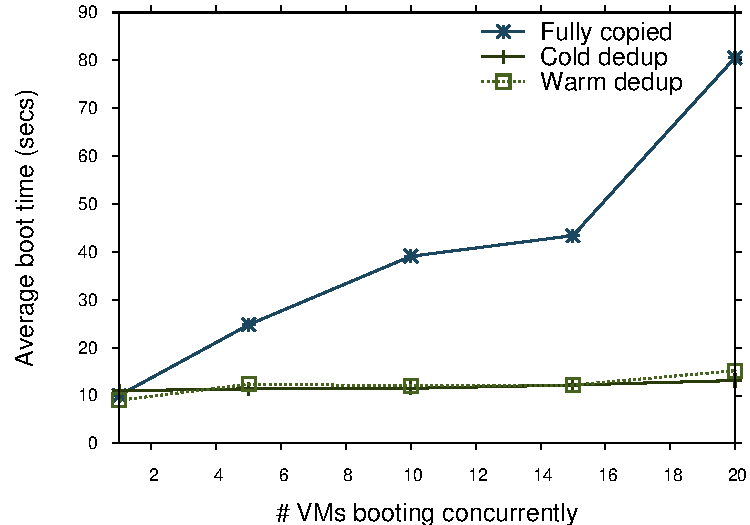
\includegraphics[scale=0.6]{figures/copied-vs-dedup.pdf}
%\vspace{-0.2in}
\caption{Windows XP VM boot up time comparison between fully
  copied VMs and deduplicated VMs.  Deduplicated VMs are booted twice
  in order to measure the impact of writing to deduplicated blocks.}
%\vspace{-0.1in}
\label{fig:copied-vs-dedup}
\end{figure}

%%%%%%%%%%%%%%%%%%%%%%%
%%%% /Figure %%%%%%%%%%
%%%%%%%%%%%%%%%%%%%%%%%

For some workloads, deduplication can actually \emph{improve} run-time
performance by decreasing the storage array cache footprint of the
workload.  To demonstrate this, we picked a common, critical,
time-limited VDI workload: booting many VMs concurrently.  VDI boot
storms can happen as part of a nightly cycle of shutting down VMs and
their hosts to conserve power, from patching guest
operating systems \emph{en masse}, from cluster fail-over, or for a
myriad of other reasons.

\XXX[Austin][Test configuration?  3-disk RAID-? on CX3-40  ``no array tuning
parameters were modified from their defaults''.]
To test the cache effects of deduplication, we compared the average time
required to boot from one to twenty VMs simultaneously between two
configurations:
%one where
(1) the VMs were each full copies of the golden VM
(much like the VDI configuration from
Section~\ref{sec:vmware-vdi-analysis}) and (2) VMs
were deduplicated copies.  The results plotted in
Figure~\ref{fig:copied-vs-dedup} show a dramatic improvement of
deduplication versus full copies, owing to the decrease in
cache footprint.

To further validate the overhead of COW specialization for a realistic
workload, we also booted the set of VMs a second time after
deduplication.  The disk images were ``cold'' the first time; they
consisted entirely of COW blocks.  The second time, any blocks
written to were already specialized and could be written to directly.
The graph shows virtually no difference between these two cases,
indicating that COW specialization overhead is not an issue for this
workload.  This is not unexpected, as there are only a few write
operations during VM boot.

% \subsubsection{VDI Workload}

% %We sought out experts at VMware familiar with VDI environments to help
% %us pick representative workloads for evaluating the effectiveness
% %of \DeDe.

% To measure the overall performance impact of \DeDe, we ran VMware's
% VDI application benchmark~\cite{vdi-benchmark}, which simulates
% corporate power users operating various productivity apps and measures
% system response time for interactive operations.  This workload is
% mostly random IO and has a write/read ratio of 0.X.  

% a workload
% used by the performance team at VMware~\cite{vdi-benchmark} to
% simulate corporate power users operating various productivity apps.

% We ran a workload used by the performance team at
% VMware~\cite{vdi-benchmark} to simulate corporate power users
% operating various productivity apps. Our characterization of the
% workload and found it to be mostly random IO with a write/read ratio
% of 0.X\%. The measurement of the test is system response time for
% interactive operations. With all virtual disks of 4~VMs completely
% deduplicated, we saw an average increase in response time across
% applications of 0.7\% (standard deviation of 0.02). Although our
% experiment only included the overheads of in-band write monitoring and
% COW, we expect that is representative due to lack of spatial locality
% in this workload.
% % (but due to experimental issues not mixed block sizes).


\subsection{Deduplication Rate}
\label{sec:dedup-rate}

While our prototype's implementation of indexing has not yet been
optimized, we measured the overall rate at which it could process
modified blocks, as well as the performance of the three main
operations performed by it: scanning the index, subdividing 1~MB
blocks into 4~KB blocks, and COW sharing duplicates.

The index scanning process operates at nearly the disk's sequential
access rate, as discussed in Section~\ref{sec:index:representation}.
At $\sim$23 bytes per index entry, our prototype can process entries for
6.6~GB of blocks \emph{per second}.  However, unlike block subdivision
and COW sharing, which require time proportional to the number of
newly shared blocks, the index scan requires time proportional to the
total number of blocks in the file system, so it is critical that this
be fast.  Once new duplicates have been discovered by the index scan,
1~MB file blocks containing any of these duplicates can be subdivided
into 4~KB blocks at 37.5~MB/sec.  Finally, these newly discovered
duplicates can be eliminated via COW sharing at 2.6~MB/sec.

The COW sharing step limits our prototype to processing $\sim$9~GB of
new \emph{shared} blocks per hour.  Unique blocks (\ie, recently
modified blocks whose hashes do not match anything in the index) can
be processed at the full index scan rate.
Furthermore, provisioning from templates, a source of large amounts of
duplicate data, can be performed directly as a COW copy (at roughly
1~GB/sec), so our deduplication rate applies only to duplicates that
arise outside of provisioning operations.
% There's actually a lot hidden in the statement we just made.  First,
% the number is an estimate based on the regular n-snap rate (0.21
% seconds/5 GB) times 256.  However, this isn't the whole story
% because we have to do the right thing in the index, which is
% complicated by unique blocks.  The best way to do this is actually
% to tell DeDe up front that the file is to be used as a template and
% that *all* blocks in it should be made shared even if there's only
% one instance.  Then there's no need to update the index or the arena
% when doing a COW copy because the source blocks will already be COW.
Still, we feel that our COW sharing rate can be significantly improved
with more profiling and optimization effort. However, even at its
current rate, the prototype can eliminate duplicates at a reasonable
rate for a VDI workload given only a few off-peak hours per day to
perform out of band deduplication.

\ignore{
  ;; Index scan rate
  (let* ((sec/gb 26.39)
         (bytes/sec (/ (* 1024 1024 1024) sec/gb))
         (entries/sec (/ bytes/sec avg-bytes/entry))
         (gb-blocks/sec (/ entries/sec 256 1024)))
    `(,sec/gb ,bytes/sec ,entries/sec ,gb-blocks/sec))
}

\XXX[
\subsection{Latency to detect duplicates}
\iffalse
\begin{notes}
  \begin{itemize}
    \item How fast can the system process write logs \& deduplicate
    \item What about writes that were missed, how long before we find
      duplicates
  \end{itemize}
\end{notes}
\fi
]
%
\incShortcut{\subsection{Hypervisor Shortcut IO}
\iffalse
\begin{notes}
  Should we add this?
  \begin{itemize}
    \item Performance improvement for reads of blocks with high ref
      counts
  \end{itemize}
\end{notes}
\fi
}
%
